\origsection{4}{分类（Classification）}
\origsubsection{4.1}{引言（Introduction）}
最后讨论剩余域 $\overline K$ 有限时单群的分类；从现在起均作这一假设。回顾，在特征零情形，此分类最早由 M. Kneser [16] 给出。表 4.2、4.3 连同 4.5 的说明，列出 $K$ 上绝对拟单群（absolutely quasi-simple groups）的所有中心同源类（central isogeny classes）。每一类群都列出以下信息；其中 $K_1$ 表示 $K$ 的非分歧闭包。

形如 ${}^aX$ 的名称：符号 $X$ 表示绝对局部 Dynkin 图 $\Delta_1$（1.11），记号同 [8，1.4.6]，但本文 $C$-$BC$ 对应于 [8] 的 $C$-$BC^{\mathrm{III}}$；$a$ 为 $\Gal(K_1/K)$ 在 $\Delta_1$ 上诱导的自同构群的阶。剩余分裂群的 $a=1$，记号中省去上标 $a$。注意，$X$ 右侧的下标为在 $K_1$ 上的相对秩，因而等于 $\Delta_1$ 的顶点数减一。若不同类型原本会得到同一名称，就用撇号、双撇号等加以区分。

按 [8] 的记号表示仿射根系（或 échelonnage）的符号：剩余分裂情形中，此符号与类型名称相同，故不单列。符号的右侧部分给出相对根系 $\Phi$ 的类型；特别地，右下标为在 $K$ 上的相对秩，因而等于相对局部 Dynkin 图 $\Delta$ 的顶点数减一。

局部指标（1.11）、相对局部 Dynkin 图 $\Delta$（1.8）及各顶点所带的整数 $d(v)$（1.8）：$\Gal(K_1/K)$ 通过 $a$ 阶循环群在 $\Delta_1$ 上的作用，基本由其在 $\Delta_1$ 顶点集中的轨道刻画。图中如下展示轨道：对应于 $\Delta$ 顶点 $v$ 的轨道 $O(v)$（1.11）的元素，紧靠排列在与 $v$ 相同的竖线上（$\Delta$ 的两个顶点位于同一竖线的少数情形，例如 ${}^2D_n$、${}^2D''_{2m}$ 等，$v\mapsto O(v)$ 的对应由图的画法应当清楚）。由于 $\overline K$ 有限，$G$ 剩余拟分裂（1.10.3），因此除了唯一的各向异性类型 ${}^dA_{d-1}$ 外，$\Delta_1$ 全部顶点都是标识顶点（1.11），无须像 [22] 那样另外圈出轨道。超特殊顶点（1.10）标以 hs，其他特殊顶点（1.9）标以 s。

按 [3]、[22] 中通常定义的型指标：为简便起见，不画出这一指标，而用 [22] 记号中的相应符号表示。回顾，这一符号除其他信息外，还含有群的绝对类型、绝对秩、相对秩（表示 $\Phi_{\mathrm{af}}$ 的符号已给出），以及 $K$ 的可分闭包的 Galois 群在通常 Dynkin 图上诱导的自同构群的阶。

$A_n$ 的内形式（inner forms）较适合用文字描述，因此相应条目以文字代替图。
\origsubsection{4.2}{剩余分裂群（Residually split groups）}
\begin{longtable}{p{.20\linewidth}p{.52\linewidth}p{.19\linewidth}}
\toprule 名称 & 局部 Dynkin 图 & 指标 [22] \\\midrule\endhead
$A_n\ (n\geq2)$ & 长度为 $n+1$ 的环，全部顶点均超特殊 & ${}^1A_{n,n}^{(1)}$\\[8pt]
$A_1$ & \begin{tikzpicture}[x=.43cm,y=.43cm,line width=.5pt]
\coordinate (n0) at (0,0);\draw(0,{0-.08})--(0,{0+.08});
\coordinate (n1) at (1,0);\draw(1,{0-.08})--(1,{0+.08});
\draw[line width=2pt](n0)--(n1);
\node[below]at($(n0)+(0,-.12)$){hs};
\node[below]at($(n1)+(0,-.12)$){hs};
\end{tikzpicture} & ${}^1A_{1,1}^{(1)}$\\[10pt]
$B_n\ (n\geq3)$ & \begin{tikzpicture}[x=.43cm,y=.43cm,line width=.5pt]
\coordinate (n0) at (0,0);\draw(0,{0-.08})--(0,{0+.08});
\coordinate (n1) at (1,0);\draw(1,{0-.08})--(1,{0+.08});
\coordinate (n2) at (2,0);\draw(2,{0-.08})--(2,{0+.08});
\coordinate (n3) at (3,0);\draw(3,{0-.08})--(3,{0+.08});
\coordinate (n4) at (4,0);\draw(4,{0-.08})--(4,{0+.08});
\coordinate (n5) at (5,0.8);\draw(5,{0.8-.08})--(5,{0.8+.08});
\coordinate (n6) at (5,-0.8);\draw(5,{-0.8-.08})--(5,{-0.8+.08});
\draw($(n0)+(0,-0.06)$)--($(n1)+(0,-0.06)$);
\draw($(n0)+(0,0.06)$)--($(n1)+(0,0.06)$);
\draw[->]($(n1)!.3!(n0)$)--($(n1)!.7!(n0)$);
\draw[solid](n1)--(n2);
\draw[dashed](n2)--(n3);
\draw[solid](n3)--(n4);
\draw[solid](n4)--(n5);
\draw[solid](n4)--(n6);
\node[below]at($(n5)+(0,-.12)$){hs};
\node[below]at($(n6)+(0,-.12)$){hs};
\end{tikzpicture} & $B_{n,n}$\\[10pt]
$B\text{-}C_n\ (n\geq3)$ & \begin{tikzpicture}[x=.43cm,y=.43cm,line width=.5pt]
\coordinate (n0) at (0,0);\draw(0,{0-.08})--(0,{0+.08});
\coordinate (n1) at (1,0);\draw(1,{0-.08})--(1,{0+.08});
\coordinate (n2) at (2,0);\draw(2,{0-.08})--(2,{0+.08});
\coordinate (n3) at (3,0);\draw(3,{0-.08})--(3,{0+.08});
\coordinate (n4) at (4,0);\draw(4,{0-.08})--(4,{0+.08});
\coordinate (n5) at (5,0.8);\draw(5,{0.8-.08})--(5,{0.8+.08});
\coordinate (n6) at (5,-0.8);\draw(5,{-0.8-.08})--(5,{-0.8+.08});
\draw($(n0)+(0,-0.06)$)--($(n1)+(0,-0.06)$);
\draw($(n0)+(0,0.06)$)--($(n1)+(0,0.06)$);
\draw[->]($(n0)!.3!(n1)$)--($(n0)!.7!(n1)$);
\draw[solid](n1)--(n2);
\draw[dashed](n2)--(n3);
\draw[solid](n3)--(n4);
\draw[solid](n4)--(n5);
\draw[solid](n4)--(n6);
\node[below]at($(n5)+(0,-.12)$){s};
\node[below]at($(n6)+(0,-.12)$){s};
\end{tikzpicture} & ${}^2A_{2n-1,n}^{(1)}$\\[10pt]
$C_n\ (n\geq2)$ & \begin{tikzpicture}[x=.43cm,y=.43cm,line width=.5pt]
\coordinate (n0) at (0,0);\draw(0,{0-.08})--(0,{0+.08});
\coordinate (n1) at (1,0);\draw(1,{0-.08})--(1,{0+.08});
\coordinate (n2) at (2,0);\draw(2,{0-.08})--(2,{0+.08});
\coordinate (n3) at (3,0);\draw(3,{0-.08})--(3,{0+.08});
\coordinate (n4) at (4,0);\draw(4,{0-.08})--(4,{0+.08});
\coordinate (n5) at (5,0);\draw(5,{0-.08})--(5,{0+.08});
\draw($(n0)+(0,-0.06)$)--($(n1)+(0,-0.06)$);
\draw($(n0)+(0,0.06)$)--($(n1)+(0,0.06)$);
\draw[->]($(n0)!.3!(n1)$)--($(n0)!.7!(n1)$);
\draw[solid](n1)--(n2);
\draw[dashed](n2)--(n3);
\draw[solid](n3)--(n4);
\draw($(n4)+(0,-0.06)$)--($(n5)+(0,-0.06)$);
\draw($(n4)+(0,0.06)$)--($(n5)+(0,0.06)$);
\draw[->]($(n5)!.3!(n4)$)--($(n5)!.7!(n4)$);
\node[below]at($(n0)+(0,-.12)$){hs};
\node[below]at($(n5)+(0,-.12)$){hs};
\end{tikzpicture} & $C_{n,n}^{(1)}$\\[10pt]
$C\text{-}B_n\ (n\geq2)$ & \begin{tikzpicture}[x=.43cm,y=.43cm,line width=.5pt]
\coordinate (n0) at (0,0);\draw(0,{0-.08})--(0,{0+.08});
\coordinate (n1) at (1,0);\draw(1,{0-.08})--(1,{0+.08});
\coordinate (n2) at (2,0);\draw(2,{0-.08})--(2,{0+.08});
\coordinate (n3) at (3,0);\draw(3,{0-.08})--(3,{0+.08});
\coordinate (n4) at (4,0);\draw(4,{0-.08})--(4,{0+.08});
\coordinate (n5) at (5,0);\draw(5,{0-.08})--(5,{0+.08});
\draw($(n0)+(0,-0.06)$)--($(n1)+(0,-0.06)$);
\draw($(n0)+(0,0.06)$)--($(n1)+(0,0.06)$);
\draw[->]($(n1)!.3!(n0)$)--($(n1)!.7!(n0)$);
\draw[solid](n1)--(n2);
\draw[dashed](n2)--(n3);
\draw[solid](n3)--(n4);
\draw($(n4)+(0,-0.06)$)--($(n5)+(0,-0.06)$);
\draw($(n4)+(0,0.06)$)--($(n5)+(0,0.06)$);
\draw[->]($(n4)!.3!(n5)$)--($(n4)!.7!(n5)$);
\node[below]at($(n0)+(0,-.12)$){s};
\node[below]at($(n5)+(0,-.12)$){s};
\end{tikzpicture} & ${}^2D_{n+1,n}^{(1)}$\\[10pt]
$C\text{-}BC_n\ (n\geq2)$ & \begin{tikzpicture}[x=.43cm,y=.43cm,line width=.5pt]
\coordinate (n0) at (0,0);\draw(0,{0-.08})--(0,{0+.08});
\coordinate (n1) at (1,0);\draw(1,{0-.08})--(1,{0+.08});
\coordinate (n2) at (2,0);\draw(2,{0-.08})--(2,{0+.08});
\coordinate (n3) at (3,0);\draw(3,{0-.08})--(3,{0+.08});
\coordinate (n4) at (4,0);\draw(4,{0-.08})--(4,{0+.08});
\coordinate (n5) at (5,0);\draw(5,{0-.08})--(5,{0+.08});
\draw($(n0)+(0,-0.06)$)--($(n1)+(0,-0.06)$);
\draw($(n0)+(0,0.06)$)--($(n1)+(0,0.06)$);
\draw[->]($(n1)!.3!(n0)$)--($(n1)!.7!(n0)$);
\draw[solid](n1)--(n2);
\draw[dashed](n2)--(n3);
\draw[solid](n3)--(n4);
\draw($(n4)+(0,-0.06)$)--($(n5)+(0,-0.06)$);
\draw($(n4)+(0,0.06)$)--($(n5)+(0,0.06)$);
\draw[->]($(n5)!.3!(n4)$)--($(n5)!.7!(n4)$);
\node[below]at($(n0)+(0,-.12)$){s};
\node[below]at($(n5)+(0,-.12)$){s};
\end{tikzpicture} & ${}^2A_{2n,n}^{(1)}$\\[10pt]
$C\text{-}BC_1$ & \begin{tikzpicture}[x=.43cm,y=.43cm,line width=.5pt]
\coordinate (n0) at (0,0);\draw(0,{0-.08})--(0,{0+.08});
\coordinate (n1) at (1,0);\draw(1,{0-.08})--(1,{0+.08});
\draw[line width=2pt](n0)--(n1);
\draw[->]($(n1)!.3!(n0)$)--($(n1)!.7!(n0)$);
\node[below]at($(n0)+(0,-.12)$){s};
\node[below]at($(n1)+(0,-.12)$){s};
\end{tikzpicture} & ${}^2A_{2,1}^{(1)}$\\[10pt]
$D_n\ (n\geq4)$ & \begin{tikzpicture}[x=.43cm,y=.43cm,line width=.5pt]
\coordinate (n0) at (-1,0.8);\draw(-1,{0.8-.08})--(-1,{0.8+.08});
\coordinate (n1) at (-1,-0.8);\draw(-1,{-0.8-.08})--(-1,{-0.8+.08});
\coordinate (n2) at (0,0);\draw(0,{0-.08})--(0,{0+.08});
\coordinate (n3) at (1,0);\draw(1,{0-.08})--(1,{0+.08});
\coordinate (n4) at (2,0);\draw(2,{0-.08})--(2,{0+.08});
\coordinate (n5) at (3,0);\draw(3,{0-.08})--(3,{0+.08});
\coordinate (n6) at (4,0.8);\draw(4,{0.8-.08})--(4,{0.8+.08});
\coordinate (n7) at (4,-0.8);\draw(4,{-0.8-.08})--(4,{-0.8+.08});
\draw[solid](n0)--(n2);
\draw[solid](n1)--(n2);
\draw[solid](n2)--(n3);
\draw[dashed](n3)--(n4);
\draw[solid](n4)--(n5);
\draw[solid](n5)--(n6);
\draw[solid](n5)--(n7);
\node[below]at($(n0)+(0,-.12)$){hs};
\node[below]at($(n1)+(0,-.12)$){hs};
\node[below]at($(n6)+(0,-.12)$){hs};
\node[below]at($(n7)+(0,-.12)$){hs};
\end{tikzpicture} & ${}^1D_{n,n}^{(1)}$\\[10pt]
$E_6$ & \begin{tikzpicture}[x=.43cm,y=.43cm,line width=.5pt]
\coordinate (n0) at (0,0);\draw(0,{0-.08})--(0,{0+.08});
\coordinate (n1) at (1,0);\draw(1,{0-.08})--(1,{0+.08});
\coordinate (n2) at (2,0);\draw(2,{0-.08})--(2,{0+.08});
\coordinate (n3) at (3,1);\draw(3,{1-.08})--(3,{1+.08});
\coordinate (n4) at (4,2);\draw(4,{2-.08})--(4,{2+.08});
\coordinate (n5) at (3,-1);\draw(3,{-1-.08})--(3,{-1+.08});
\coordinate (n6) at (4,-2);\draw(4,{-2-.08})--(4,{-2+.08});
\draw[solid](n0)--(n1);
\draw[solid](n1)--(n2);
\draw[solid](n2)--(n3);
\draw[solid](n3)--(n4);
\draw[solid](n2)--(n5);
\draw[solid](n5)--(n6);
\node[below]at($(n0)+(0,-.12)$){hs};
\node[below]at($(n4)+(0,-.12)$){hs};
\node[below]at($(n6)+(0,-.12)$){hs};
\end{tikzpicture} & ${}^1E_{6,6}^0$\\[10pt]
$E_7$ & \begin{tikzpicture}[x=.43cm,y=.43cm,line width=.5pt]
\coordinate (n0) at (0,0);\draw(0,{0-.08})--(0,{0+.08});
\coordinate (n1) at (1,0);\draw(1,{0-.08})--(1,{0+.08});
\coordinate (n2) at (2,0);\draw(2,{0-.08})--(2,{0+.08});
\coordinate (n3) at (3,0);\draw(3,{0-.08})--(3,{0+.08});
\coordinate (n4) at (4,0);\draw(4,{0-.08})--(4,{0+.08});
\coordinate (n5) at (5,0);\draw(5,{0-.08})--(5,{0+.08});
\coordinate (n6) at (6,0);\draw(6,{0-.08})--(6,{0+.08});
\coordinate (n7) at (3,1);\draw(3,{1-.08})--(3,{1+.08});
\draw[solid](n0)--(n1);
\draw[solid](n1)--(n2);
\draw[solid](n2)--(n3);
\draw[solid](n3)--(n4);
\draw[solid](n4)--(n5);
\draw[solid](n5)--(n6);
\draw[solid](n3)--(n7);
\node[below]at($(n0)+(0,-.12)$){hs};
\node[below]at($(n6)+(0,-.12)$){hs};
\end{tikzpicture} & $E_{7,7}^0$\\[10pt]
$E_8$ & \begin{tikzpicture}[x=.43cm,y=.43cm,line width=.5pt]
\coordinate (n0) at (0,0);\draw(0,{0-.08})--(0,{0+.08});
\coordinate (n1) at (1,0);\draw(1,{0-.08})--(1,{0+.08});
\coordinate (n2) at (2,0);\draw(2,{0-.08})--(2,{0+.08});
\coordinate (n3) at (3,0);\draw(3,{0-.08})--(3,{0+.08});
\coordinate (n4) at (4,0);\draw(4,{0-.08})--(4,{0+.08});
\coordinate (n5) at (5,0);\draw(5,{0-.08})--(5,{0+.08});
\coordinate (n6) at (6,0);\draw(6,{0-.08})--(6,{0+.08});
\coordinate (n7) at (7,0);\draw(7,{0-.08})--(7,{0+.08});
\coordinate (n8) at (5,1);\draw(5,{1-.08})--(5,{1+.08});
\draw[solid](n0)--(n1);
\draw[solid](n1)--(n2);
\draw[solid](n2)--(n3);
\draw[solid](n3)--(n4);
\draw[solid](n4)--(n5);
\draw[solid](n5)--(n6);
\draw[solid](n6)--(n7);
\draw[solid](n5)--(n8);
\node[below]at($(n0)+(0,-.12)$){hs};
\end{tikzpicture} & $E_{8,8}^0$\\[10pt]
$F_4$ & \begin{tikzpicture}[x=.43cm,y=.43cm,line width=.5pt]
\coordinate (n0) at (0,0);\draw(0,{0-.08})--(0,{0+.08});
\coordinate (n1) at (1,0);\draw(1,{0-.08})--(1,{0+.08});
\coordinate (n2) at (2,0);\draw(2,{0-.08})--(2,{0+.08});
\coordinate (n3) at (3,0);\draw(3,{0-.08})--(3,{0+.08});
\coordinate (n4) at (4,0);\draw(4,{0-.08})--(4,{0+.08});
\draw[solid](n0)--(n1);
\draw[solid](n1)--(n2);
\draw($(n2)+(0,-0.06)$)--($(n3)+(0,-0.06)$);
\draw($(n2)+(0,0.06)$)--($(n3)+(0,0.06)$);
\draw[->]($(n2)!.3!(n3)$)--($(n2)!.7!(n3)$);
\draw[solid](n3)--(n4);
\node[below]at($(n0)+(0,-.12)$){hs};
\end{tikzpicture} & $F_{4,4}^0$\\[10pt]
$F_4^{\mathrm I}$ & \begin{tikzpicture}[x=.43cm,y=.43cm,line width=.5pt]
\coordinate (n0) at (0,0);\draw(0,{0-.08})--(0,{0+.08});
\coordinate (n1) at (1,0);\draw(1,{0-.08})--(1,{0+.08});
\coordinate (n2) at (2,0);\draw(2,{0-.08})--(2,{0+.08});
\coordinate (n3) at (3,0);\draw(3,{0-.08})--(3,{0+.08});
\coordinate (n4) at (4,0);\draw(4,{0-.08})--(4,{0+.08});
\draw[solid](n0)--(n1);
\draw[solid](n1)--(n2);
\draw($(n2)+(0,-0.06)$)--($(n3)+(0,-0.06)$);
\draw($(n2)+(0,0.06)$)--($(n3)+(0,0.06)$);
\draw[->]($(n3)!.3!(n2)$)--($(n3)!.7!(n2)$);
\draw[solid](n3)--(n4);
\node[below]at($(n0)+(0,-.12)$){s};
\end{tikzpicture} & ${}^2E_{6,4}^2$\\[10pt]
$G_2$ & \begin{tikzpicture}[x=.43cm,y=.43cm,line width=.5pt]
\coordinate (n0) at (0,0);\draw(0,{0-.08})--(0,{0+.08});
\coordinate (n1) at (1,0);\draw(1,{0-.08})--(1,{0+.08});
\coordinate (n2) at (2,0);\draw(2,{0-.08})--(2,{0+.08});
\draw[solid](n0)--(n1);
\draw($(n1)+(0,-0.08)$)--($(n2)+(0,-0.08)$);
\draw($(n1)+(0,0)$)--($(n2)+(0,0)$);
\draw($(n1)+(0,0.08)$)--($(n2)+(0,0.08)$);
\draw[->]($(n1)!.3!(n2)$)--($(n1)!.7!(n2)$);
\node[below]at($(n0)+(0,-.12)$){hs};
\end{tikzpicture} & $G_{2,2}$\\[10pt]
$G_2^{\mathrm I}$ & \begin{tikzpicture}[x=.43cm,y=.43cm,line width=.5pt]
\coordinate (n0) at (0,0);\draw(0,{0-.08})--(0,{0+.08});
\coordinate (n1) at (1,0);\draw(1,{0-.08})--(1,{0+.08});
\coordinate (n2) at (2,0);\draw(2,{0-.08})--(2,{0+.08});
\draw[solid](n0)--(n1);
\draw($(n1)+(0,-0.08)$)--($(n2)+(0,-0.08)$);
\draw($(n1)+(0,0)$)--($(n2)+(0,0)$);
\draw($(n1)+(0,0.08)$)--($(n2)+(0,0.08)$);
\draw[->]($(n2)!.3!(n1)$)--($(n2)!.7!(n1)$);
\node[below]at($(n0)+(0,-.12)$){s};
\end{tikzpicture} & ${}^3D_{4,2}\text{ 或 }{}^6D_{4,2}$\\[10pt]
\bottomrule
\end{longtable}
\origsubsection{4.3}{非剩余分裂群（Nonresidually split groups）}
下表中间的复杂数学图据原书第 62--66 页逐行裁切；其余列重排。各局部指标的上图表示绝对图及 Galois 轨道，下图表示相对局部 Dynkin 图。轨道的叠合、分叉和多重箭头均保留原图。
\begin{longtable}{p{.17\linewidth}p{.15\linewidth}p{.40\linewidth}p{.18\linewidth}}
\toprule 名称 & 仿射根系（[8，1.4.6]） & 局部指标及相对局部 Dynkin 图 & 指标 [22]\\\midrule\endhead
${}^dA_{md-1}$，$m\geq3,d\geq2$ & $A_{m-1}$ & 绝对局部 Dynkin 图 $\Delta_1$ 是长度为 $md$ 的环，$\Gal(K_1/K)$ 通过由环的一个旋转生成的 $d$ 阶循环群在其上作用。相对图是长度为 $m$ 的环，全部顶点均特殊但不超特殊，且带数 $d$。 & ${}^1A_{md-1,m-1}^{(d)}$\\[8pt]
${}^dA_{2d-1}$，$d\geq2$ & $A_1$ & $\Delta_1$ 如上，$m=2$；$\Delta$ 是一条粗边，两端均标 s、带数 $d$。 & ${}^1A_{2d-1,1}^{(d)}$\\[8pt]
${}^dA_{d-1}$，$d\geq2$ & $\varnothing$ & $\Delta_1$ 如上，$m=1$；或当 $d=2$ 时，由一条粗边组成，两端点被 $\Gal(K_1/K)$ 置换；$\Delta=\varnothing$。 & ${}^1A_{d-1,0}^{(d)}$\\[8pt]
${}^2A^{\prime}_{2m-1}\ (m\geq2)$ & $C_m$ & 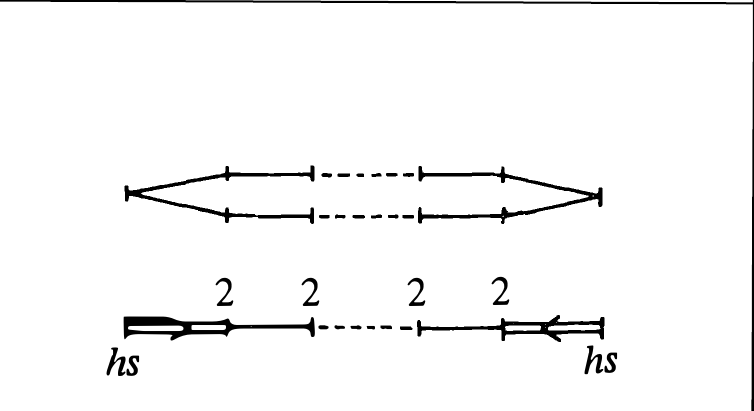
\includegraphics[width=\linewidth]{figures/02-class-66-1-066.png} & ${}^2A_{2m-1,m}^{(1)}$\\[8pt]
${}^2A^{\prime\prime}_{2m-1}\ (m\geq3)$ & $C\text{-}BC_{m-1}^{\mathrm{II}}$ & 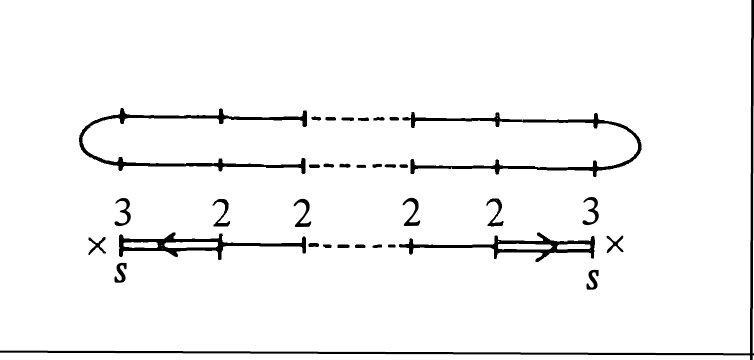
\includegraphics[width=\linewidth]{figures/02-class-66-2-066.png} & ${}^2A_{2m-1,m-1}^{(1)}$\\[8pt]
${}^2A^{\prime\prime}_3$ & $C\text{-}BC_1^{\mathrm{II}}$ & 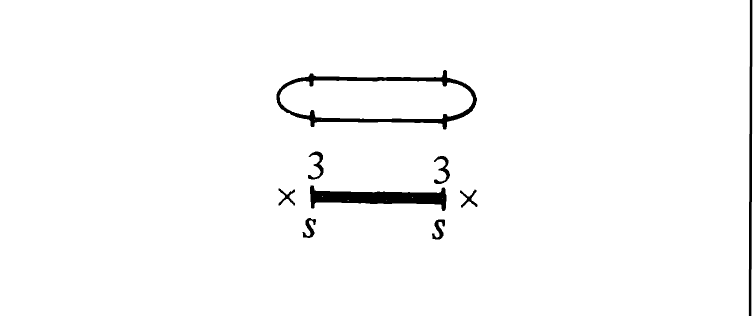
\includegraphics[width=\linewidth]{figures/02-class-66-3-066.png} & ${}^2A_{3,1}^{(1)}$\\[8pt]
${}^2A^{\prime}_{2m}\ (m\geq2)$ & $C\text{-}BC_m^{\mathrm{IV}}$ & 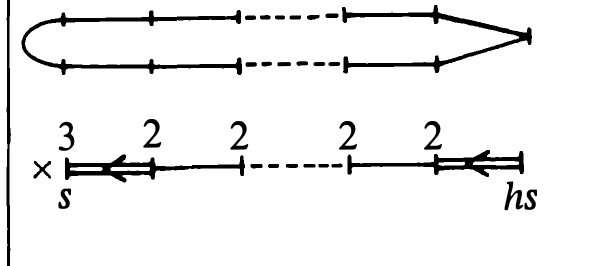
\includegraphics[width=\linewidth]{figures/02-class-67-1-067.png} & ${}^2A_{2m,m}^{(1)}$\\[8pt]
${}^2A^{\prime}_2$ & $C\text{-}BC_1^{\mathrm{IV}}$ & 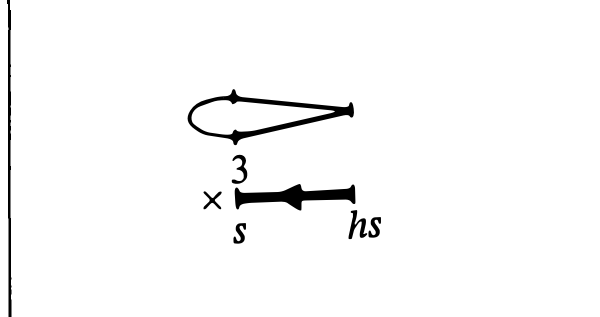
\includegraphics[width=\linewidth]{figures/02-class-67-2-067.png} & ${}^2A_{2,1}^{(1)}$\\[8pt]
${}^2B_n\ (n\geq3)$ & $C\text{-}B_{n-1}$ & 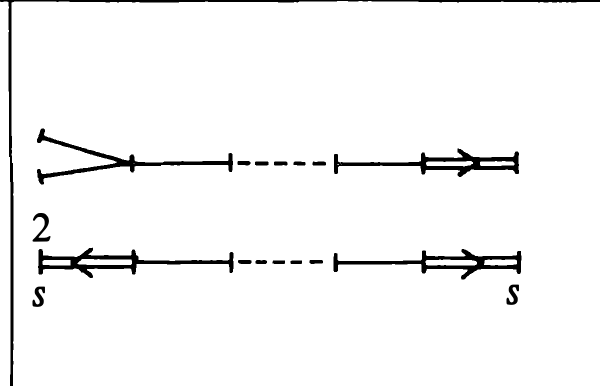
\includegraphics[width=\linewidth]{figures/02-class-67-3-067.png} & $B_{n,n-1}$\\[8pt]
${}^2B\text{-}C_n\ (n\geq3)$ & $C\text{-}BC_{n-1}^{\mathrm{III}}$ & 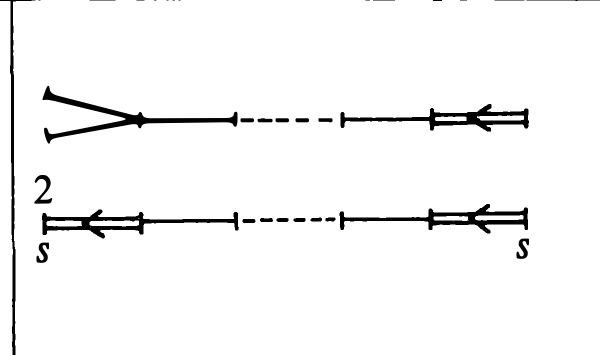
\includegraphics[width=\linewidth]{figures/02-class-67-4-067.png} & ${}^2A_{2n-1,n-1}^{(1)}$\\[8pt]
${}^2C_{2m-1}\ (m\geq3)$ & $C\text{-}BC_{m-1}^{\mathrm{IV}}$ & 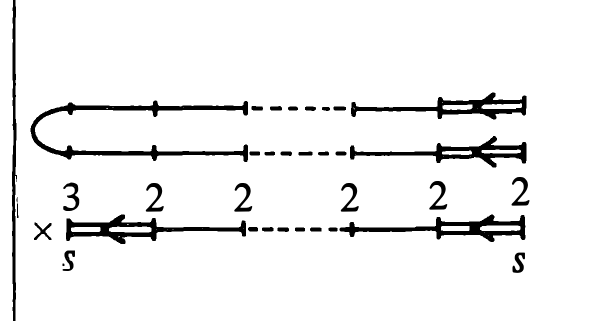
\includegraphics[width=\linewidth]{figures/02-class-67-5-067.png} & $C_{2m-1,m-1}^{(2)}$\\[8pt]
${}^2C_3$ & $C\text{-}BC_1^{\mathrm{IV}}$ & 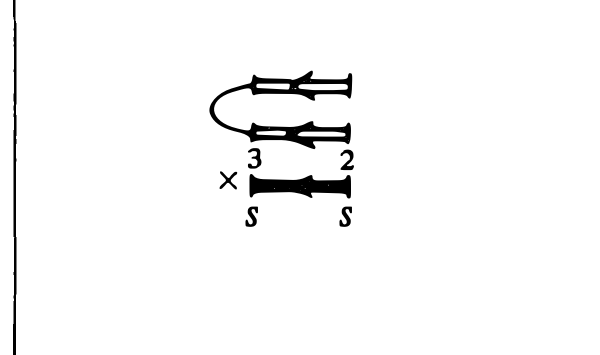
\includegraphics[width=\linewidth]{figures/02-class-67-6-067.png} & $C_{3,1}^{(2)}$\\[8pt]
${}^2C_{2m}\ (m\geq2)$ & $C_m$ & 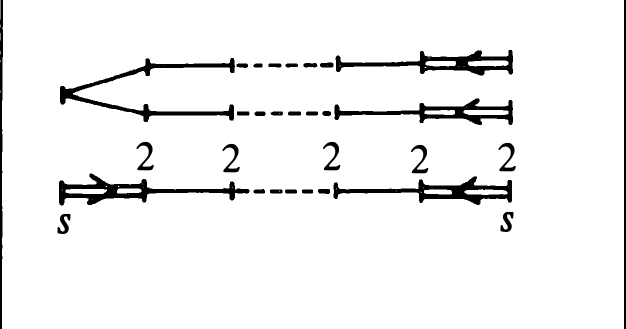
\includegraphics[width=\linewidth]{figures/02-class-68-1-068.png} & $C_{2m,m}^{(2)}$\\[8pt]
${}^2C_2$ & $A_1$ & 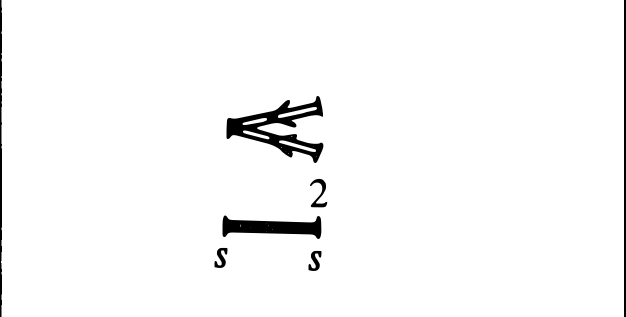
\includegraphics[width=\linewidth]{figures/02-class-68-2-068.png} & $C_{2,1}^{(2)}$\\[8pt]
${}^2C\text{-}B_{2m-1}\ (m\geq3)$ & $C\text{-}BC_{m-1}^{\mathrm I}$ & 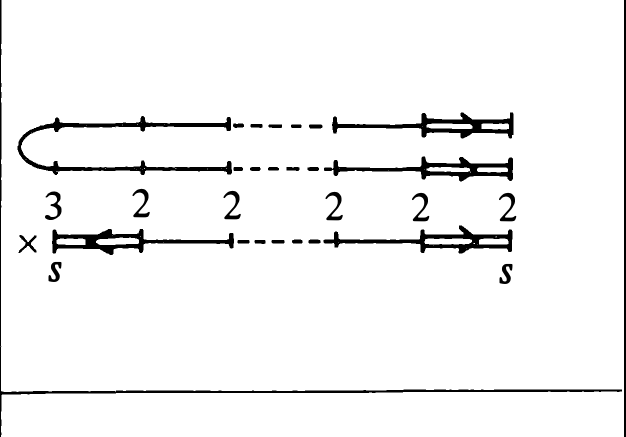
\includegraphics[width=\linewidth]{figures/02-class-68-3-068.png} & ${}^2D_{2m,m-1}^{(2)}$\\[8pt]
${}^2C\text{-}B_3$ & $C\text{-}BC_1^{\mathrm I}$ & 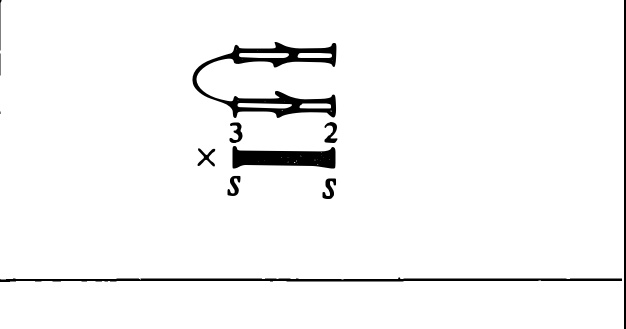
\includegraphics[width=\linewidth]{figures/02-class-68-4-068.png} & ${}^2D_{4,1}^{(2)}$\\[8pt]
${}^2C\text{-}B_{2m}\ (m\geq2)$ & $C\text{-}BC_m^{\mathrm{III}}$ & 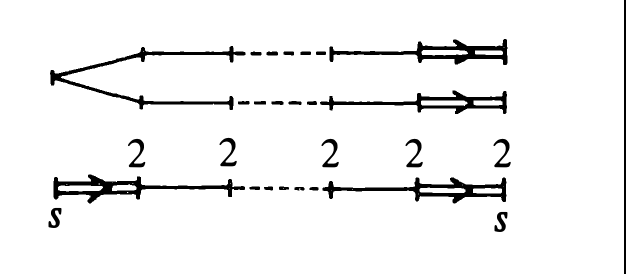
\includegraphics[width=\linewidth]{figures/02-class-68-5-068.png} & ${}^2D_{2m+1,m}^{(2)}$\\[8pt]
${}^2C\text{-}B_2$ & $C\text{-}BC_1^{\mathrm{III}}$ & 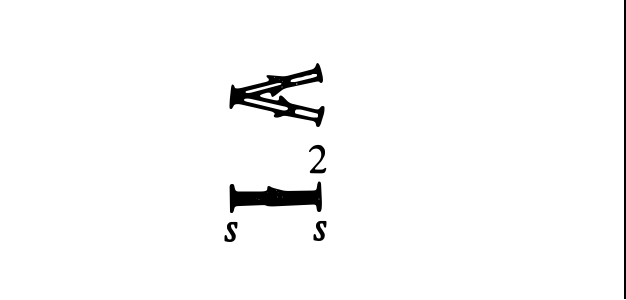
\includegraphics[width=\linewidth]{figures/02-class-68-6-068.png} & ${}^2D_{3,1}^{(2)}$\\[8pt]
${}^2D_n\ (n\geq4)$ & $B_{n-1}$ & 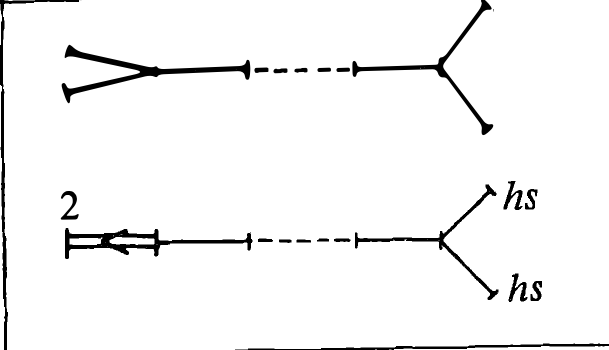
\includegraphics[width=\linewidth]{figures/02-class-69-1-069.png} & ${}^2D_{n,n-1}^{(1)}$\\[8pt]
${}^2D^{\prime}_n\ (n\geq4)$ & $C\text{-}B_{n-2}$ & 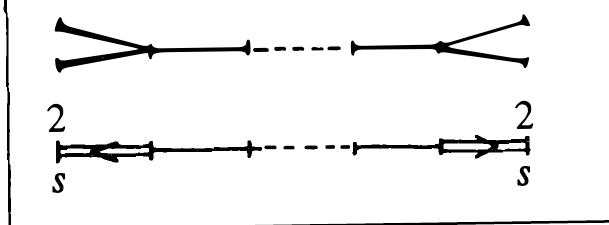
\includegraphics[width=\linewidth]{figures/02-class-69-2-069.png} & ${}^1D_{n,n-2}^{(1)}$\\[8pt]
${}^2D^{\prime\prime}_{2m}\ (m\geq3)$ & $B\text{-}C_m$ & 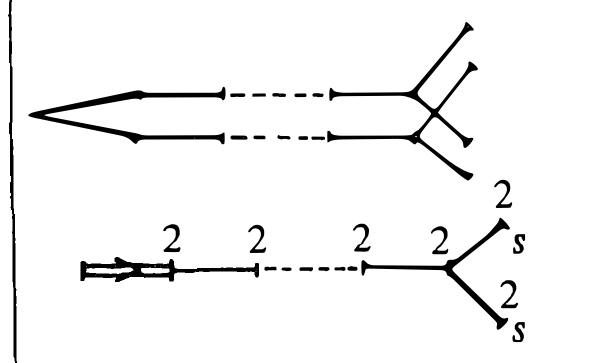
\includegraphics[width=\linewidth]{figures/02-class-69-3-069.png} & ${}^1D_{2m,m}^{(2)}$\\[8pt]
${}^2D^{\prime\prime}_{2m+1}\ (m\geq3)$ & $B\text{-}BC_m$ & 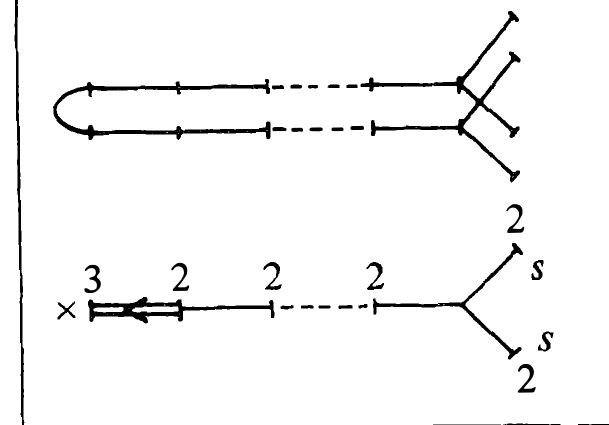
\includegraphics[width=\linewidth]{figures/02-class-69-4-069.png} & ${}^2D_{2m+1,m}^{(2)}$\\[8pt]
${}^2D^{\prime\prime}_5$ & $B\text{-}BC_2$ & 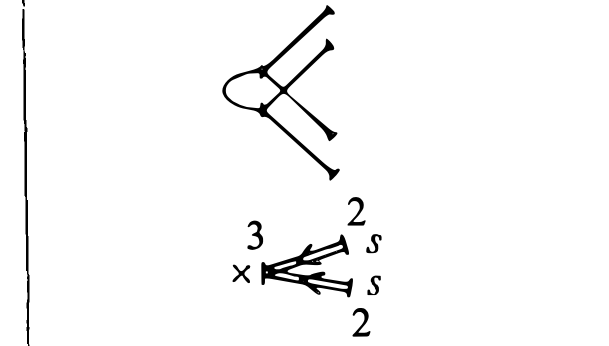
\includegraphics[width=\linewidth]{figures/02-class-69-5-069.png} & ${}^2D_{5,2}^{(2)}$\\[8pt]
${}^3D_4$ & $G_2$ & 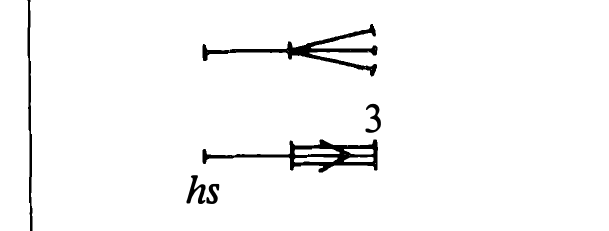
\includegraphics[width=\linewidth]{figures/02-class-69-6-069.png} & ${}^3D_{4,2}$\\[8pt]
${}^4D_{2m}\ (m\geq3)$ & $C\text{-}BC_{m-1}^{\mathrm{III}}$ & 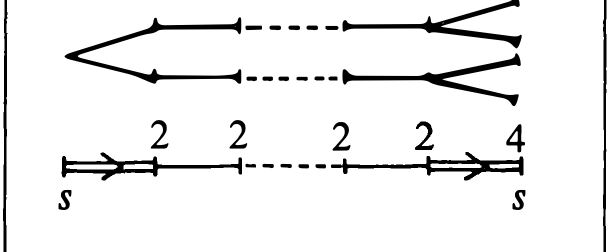
\includegraphics[width=\linewidth]{figures/02-class-70-1-070.png} & ${}^2D_{2m,m-1}^{(2)}$\\[8pt]
${}^4D_4$ & $C\text{-}BC_1^{\mathrm{III}}$ & 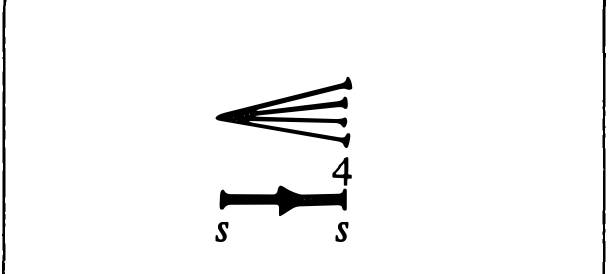
\includegraphics[width=\linewidth]{figures/02-class-70-2-070.png} & ${}^2D_{4,1}^{(2)}$\\[8pt]
${}^4D_{2m+1}\ (m\geq3)$ & $C\text{-}BC_{m-1}^{\mathrm I}$ & 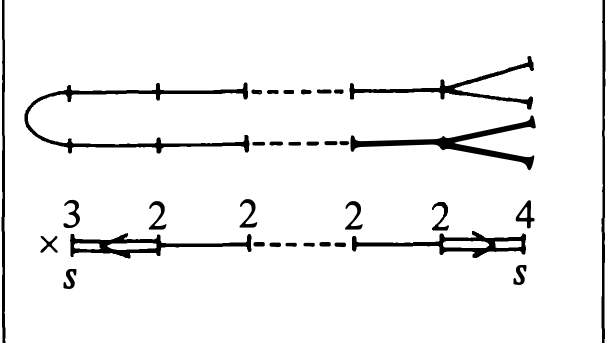
\includegraphics[width=\linewidth]{figures/02-class-70-3-070.png} & ${}^1D_{2m+1,m-1}^{(2)}$\\[8pt]
${}^4D_5$ & $C\text{-}BC_1^{\mathrm I}$ & 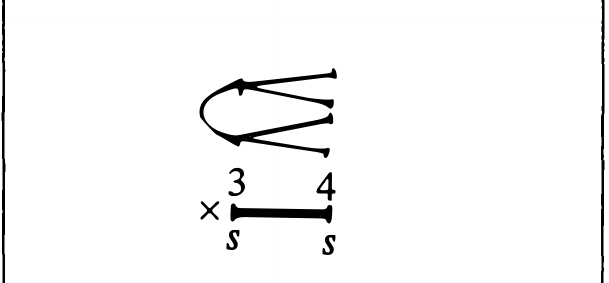
\includegraphics[width=\linewidth]{figures/02-class-70-4-070.png} & ${}^1D_{5,1}^{(2)}$\\[8pt]
${}^2E_6$ & $F_4$ & 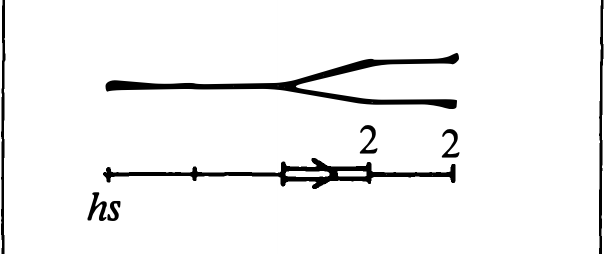
\includegraphics[width=\linewidth]{figures/02-class-70-5-070.png} & ${}^2E_{6,4}^2$\\[8pt]
${}^3E_6$ & $G_2^{\mathrm I}$ & 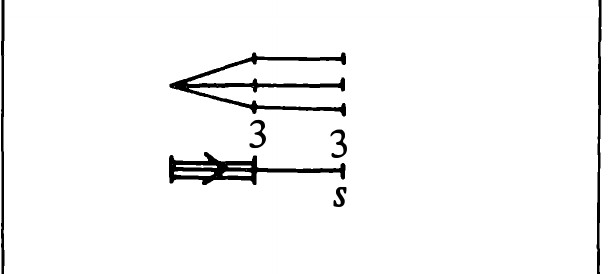
\includegraphics[width=\linewidth]{figures/02-class-70-6-070.png} & ${}^1E_{6,2}^{16}$\\[8pt]
${}^2E_7$ & $F_4^{\mathrm I}$ & 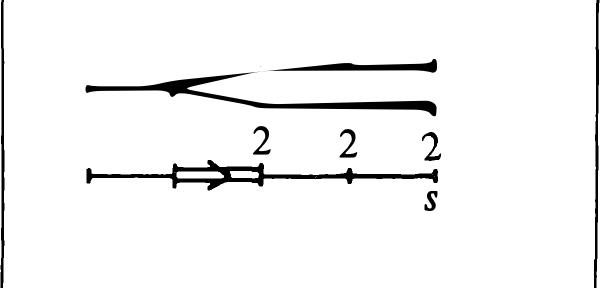
\includegraphics[width=\linewidth]{figures/02-class-70-7-070.png} & $E_{7,4}^9$\\[8pt]
\bottomrule
\end{longtable}
\noindent ${}^2D''_5$ 一行的仿射根系 $B$-$BC_2$：原注指出，这一 échelonnage 在 [8，第 29 页] 的表中遗漏。
\origsubsection{4.4}{解释（Interpretation）}
下面用经典术语重新表述这一分类，为 $K$ 上绝对拟单群的每个中心同源类选取一个代表，并在每种情形给出相应类型名称，记号同表 4.2、4.3 第一列。

$K$ 上 $d^2$ 维中心除代数的特殊线性群（special linear group）$\SL_m$，$md\geq2$。类型为 ${}^dA_{md-1}$。

$K$ 的二次扩张 $L$ 上 $r$ 个变量的 Hermite 型 $h$（$r\geq3$）、Witt 指标（Witt index）为 $r'$ 的特殊酉群（special unitary group）$\operatorname{SU}(h)$。如果 $L/K$ 分歧，假设 $r\ne4$；因为 $r=4$ 的情形，在 $r'=2$ 或 $1$ 时，分别更适合用六个变量的通常特殊正交群，或三个变量的四元数特殊正交群表示。若型 $h$ 分裂，则当 $L/K$ 非分歧时类型为 ${}^2A'_{r-1}$；否则为 $C$-$BC_n$（$r=2n+1$）或 $B$-$C_n$（$r=2n$）。若 $h$ 不分裂，则 $r=2r'+2$，当 $L/K$ 非分歧或分歧时，类型分别为 ${}^2A''_{r-1}$ 或 ${}^2B$-$C_{r'+1}$。

$K$ 上 $r$ 个变量的二次型 $q$（$r\geq6$）、Witt 指标为 $r'$ 的特殊正交群（special orthogonal group）$\operatorname{SO}(q)$。若 $r$ 为偶数，以 $L$ 表示 $q$ 的偶 Clifford 代数（even Clifford algebra）的中心，它同构于 $K\oplus K$（型 $q$ 的判别式为一或 Arf 不变量为零），或为 $K$ 的二次扩张。若 $L/K$ 非分歧（特别是 $L=K\oplus K$），假设 $r\ne6$，因为 $r=6$ 更适合由四个变量的特殊酉群表示。若 $r=2r'$（$2r'+1$），类型为 $D_{r'}$（$B_{r'}$）。若 $r=2r'+2$，则 $L$ 为 $K$ 的二次扩张，当 $L/K$ 非分歧或分歧时，类型分别为 ${}^2D_{r'+1}$ 或 $C$-$B_{r'}$。最后，若 $r=2r'+3$（$2r'+4$），类型为 ${}^2B_{r'+1}$（${}^2D'_{r'+2}$）。

$2n\geq4$ 个变量的辛群（symplectic group）类型为 $C_n$。

关于标准对合（standard involution）的 $r$ 个变量的四元数 Hermite 型（quaternion hermitian form）的特殊酉群，$r\geq2$。Witt 指标总是最大的，类型为 ${}^2C_r$。

关于四元数代数对合 $\sigma$ 的 $r$ 个变量的四元数 $\sigma$ 二次型（quaternionic $\sigma$-quadratic form）的特殊正交群 $\operatorname{SO}(q)$，$r\geq3$，其中该对合的对称元素空间为三维（见 [21]、[23]；若 $\operatorname{char}K\ne2$，“$\sigma$ 二次”即“$\sigma$ Hermite”，该群也是一个关于标准对合的反 Hermite 型的特殊酉群）。令 $r'$ 为型的 Witt 指标，$L$ 为其“偶”Clifford 代数 $\operatorname{Cl}(q)$ 的中心（见 [21]）。若 $L/K$ 非分歧（特别是 $L\simeq K\oplus K$），假设 $r\ne3$，因为 $r=3$ 更适合由四个变量的特殊酉群表示；若进一步 $r=2r'$，还假设 $r\ne4$，因为 $r=2r'=4$ 通过三重性原理（triality principle），更适合由八个变量、Witt 指标为 $2$ 的通常特殊正交群表示。总有 $2r'\leq r\leq2r'+3$。若 $r=2r'$，则 $L\simeq K\oplus K$，群类型为 ${}^2D''_r$。若 $r=2r'+1$（$2r'+2$），则 $L$ 为 $K$ 的二次扩张；当 $L/K$ 非分歧或分歧时，类型分别为 ${}^2D''_r$（${}^4D_r$）或 ${}^2C$-$B_{r-1}$。若 $r=2r'+3$，则 $L\simeq K\oplus K$，类型为 ${}^4D_r$。

拟分裂三重性 $D_4$（quasi-split triality $D_4$）。令 $L$ 为分裂域，它是三次循环扩张，或 Galois 群为 $\mathfrak S_3$ 的六次 Galois 扩张。若 $L/K$ 非分歧（因而为三次循环扩张），类型为 ${}^3D_4$；否则为 $G_2^{\mathrm I}$。

分裂例外群（split exceptional groups）。类型名称与其绝对类型相同，即 $G_2$、$F_4$、$E_6$、$E_7$、$E_8$。

$E_6$ 型拟分裂群。其类型在二次分裂域 $L$ 非分歧或分歧时，分别为 ${}^2E_6$ 或 $F_4^{\mathrm I}$。

$E_6$、$E_7$ 型非拟分裂群。它们分别是借助维数为 $9$、$4$ 的中心除代数构造的 $E_6$、$E_7$ 的形式；类型为 ${}^3E_6$、${}^2E_7$。
\origsubsection{4.5}{不变量（Invariants）}
表 4.2、4.3 所列的全部群类型，在任何满足本文假设且剩余域有限的 $K$ 上都存在。给定名称对应的中心同源类总是唯一，只有下述例外。

$d\geq5$ 时，${}^dA_{md-1}$ 型的同源类，由 $K$ 上维数为 $d^2$ 的互为反代数的中心除代数对分类；因而其数目为 $\frac12\varphi(d)$，其中 $\varphi$ 为 Euler 函数。

$B$-$C_n$、${}^2B$-$C_n$、$C$-$B_n$、${}^2C$-$B_n$、$C$-$BC_n$ 及 $F_4^{\mathrm I}$ 型的同源类，由 $K$ 的分歧二次扩张分类，即 4.4 中一直记为 $L$ 的扩张。

$G_2^{\mathrm I}$ 型的群，由 $K$ 的 Galois 扩张 $L$ 分类，其中 $L/K$ 为三次循环扩张，或六次非循环扩张。\footnote{\textbf{译者注（本次校订）：}这里还须要求 $L/K$ 分歧。按照4.4的区分，非分歧三次循环扩张对应的是 ${}^3D_4$，而非 $G_2^{\mathrm I}$。}
\origsubsection{4.6}{分类工具包（The classification kit）}
下面的规律提供了一种重建分类的便捷方法。首先，除 ${}^dA_{d-1}$ 外，表 4.2、4.3 的每种类型均由局部 Dynkin 图及其所带整数 $d(v)$ 完全刻画。现在考虑一个秩（顶点数）至少为三的仿射型连通 Coxeter 图，为每个顶点附上一个整数，在某些顶点标叉（也可以一个都不标），并用箭头将每条双线或三线定向。则存在半单群 $G$，其相对局部 Dynkin 图为所得图、且给定整数为 $d(v)$，当且仅当由每对顶点构成的所有子图均属于下列类型之一。这些图代表相对秩为二的拟分裂群的通常 Dynkin 图：
\begin{center}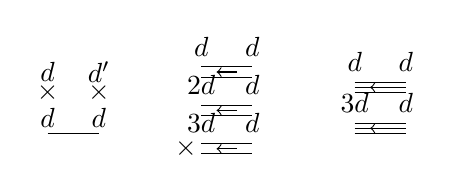
\begin{tikzpicture}[x=.65cm,y=.65cm]
\node at(0,1.1){$d$};\node at(1,1.1){$d'$};\node at(0,.7){$\times$};\node at(1,.7){$\times$};
\draw(0,-.1)--(1,-.1);\node at(0,.2){$d$};\node at(1,.2){$d$};
\foreach\y/\a in {1.1/d,.35/2d,-.4/3d}{
\draw(3,\y-.1)--(4,\y-.1) (3,\y+.1)--(4,\y+.1);\draw[->](3.7,\y)--(3.3,\y);
\node[above]at(3,\y+.12){$\a$};\node[above]at(4,\y+.12){$d$};}
\node at(2.7,-.4){$\times$};
\foreach\y/\a in {.8/d,0/3d}{
\draw(6,\y-.1)--(7,\y-.1) (6,\y)--(7,\y) (6,\y+.1)--(7,\y+.1);\draw[->](6.7,\y)--(6.3,\y);
\node[above]at(6,\y+.12){$\a$};\node[above]at(7,\y+.12){$d$};}
\end{tikzpicture}
\end{center}
而且，群 $G$ 可选为绝对拟单，当且仅当各整数 $d(v)$ 互素，或底层 Coxeter 图为环。至于相对秩为一、底层 Coxeter 图为粗边的类型，它们可作为更高秩类型的“极限情形”得到，这里不再详述。
\begin{thebibliography}{99}
\bibitem[1]{c02-1} A. Borel, \emph{Admissible representations of a semi-simple group over a local field with vectors fixed under an Iwahori subgroup}, Invent. Math. 35 (1976), 233--259.
\bibitem[2]{c02-2} A. Borel et J.-P. Serre, \emph{Cohomologie d'immeubles et de groupes S-arithmétiques}, Topology 15 (1976), 211--232.
\bibitem[3]{c02-3} A. Borel et J. Tits, \emph{Groupes réductifs}, Publ. Math. Inst. Hautes Études Scientifiques 27 (1965), 55--150.
\bibitem[4]{c02-4} A. Borel et J. Tits, \emph{Compléments à l'article ``Groupes réductifs''}, Publ. Math. Inst. Hautes Études Scientifiques 41 (1972), 253--276.
\bibitem[5]{c02-5} N. Bourbaki, \emph{Groupes et algèbres de Lie}, Chap. IV, V, VI, Hermann, Paris, 1968.
\bibitem[6]{c02-6} F. Bruhat et J. Tits, (a) \emph{BN-paires de type affine et données radicielles}, C. R. Acad. Sci. Paris 263 (1966), 598--601; (b) \emph{Groupes simples résiduellement déployés sur un corps local}, 同刊，766--768; (c) \emph{Groupes algébriques simples sur un corps local}, 同刊，822--825; (d) \emph{Groupes algébriques simples sur un corps local: cohomologie galoisienne, décompositions d'Iwasawa et de Cartan}, 同刊，867--869.
\bibitem[7]{c02-7} F. Bruhat et J. Tits, \emph{Groupes algébriques simples sur un corps local}, Proc. Conf. on Local Fields (Driebergen, 1966), Springer, New York, 1967, pp. 23--36.
\bibitem[8]{c02-8} F. Bruhat et J. Tits, \emph{Groupes réductifs sur un corps local. I, Données radicielles valuées}, Publ. Math. Inst. Hautes Études Scientifiques 41 (1972), 5--251.
\bibitem[9]{c02-9} F. Bruhat et J. Tits, \emph{Groupes réductifs sur un corps local. II, Schémas en groupes}（准备中）。
\bibitem[10]{c02-10} C. Chevalley, \emph{Sur certains groupes simples}, Tôhoku Math. J. 7 (1955), 14--66.
\bibitem[11]{c02-11} M. Demazure et A. Grothendieck, \emph{Schémas en groupes. III}, Sém. Géom. Alg. 1962/64, Lecture Notes in Math., vol. 153, Springer, New York, 1970.
\bibitem[12]{c02-12} O. Goldman et N. Iwahori, \emph{The space of p-adic norms}, Acta Math. 109 (1963), 137--177.
\bibitem[13]{c02-13} H. Hijikata, \emph{On the arithmetic of p-adic Steinberg groups}, 油印讲义，Yale Univ., 1964.
\bibitem[14]{c02-14} H. Hijikata, \emph{On the structure of semi-simple algebraic groups over valuation fields. I}, Japan. J. Math. 1 (1975), 225--300.
\bibitem[15]{c02-15} N. Iwahori and H. Matsumoto, \emph{On some Bruhat decomposition and the structure of the Hecke ring of p-adic Chevalley groups}, Publ. Math. Inst. Hautes Études Scientifiques 25 (1965), 5--48.
\bibitem[16]{c02-16} M. Kneser, \emph{Galois-Kohomologie halbeinfacher algebraischer Gruppen über p-adischen Körpern}, Math. Z. 88 (1965), 40--47; 89 (1965), 250--272.
\bibitem[17]{c02-17} I. G. MacDonald, \emph{Affine root systems and Dedekind's $\eta$ function}, Invent. Math. 15 (1972), 91--143.
\bibitem[18]{c02-18} G. Prasad, \emph{Lattices in semi-simple groups over local fields}, Advances in Math.（即将发表）。
\bibitem[19]{c02-19} G. Rousseau, \emph{Immeubles des groupes réductifs sur les corps locaux}, 博士论文，Paris XI (1977).
\bibitem[20]{c02-20} T. A. Springer, \emph{Reductive groups}, 本论文集，第 1 册，第 3--27 页。
\bibitem[21]{c02-21} J. Tits, \emph{Formes quadratiques, groupes orthogonaux et algèbres de Clifford}, Invent. Math. 5 (1968), 19--41.
\bibitem[22]{c02-22} J. Tits, \emph{Classification of algebraic semisimple groups}, Proc. Summer Inst. on Algebraic Groups and Discontinuous Groups (Boulder, 1965), Proc. Sympos. Pure Math., vol. 9, Amer. Math. Soc., Providence, R. I., 1966, pp. 33--62.
\bibitem[23]{c02-23} J. Tits, \emph{Buildings of spherical type and finite BN-pairs}, Lecture Notes in Math., vol. 386, Springer, New York, 1974.
\bibitem[24]{c02-24} J. Tits, \emph{On buildings and their applications}, Proc. Internat. Congr. Math. (Vancouver, 1974), vol. 1, Canad. Math. Congr., 1975, pp. 209--220.
\bibitem[25]{c02-25} J. Tits, \emph{Résumé de cours}, Annuaire du Collège de France pour 1975--1976, pp. 49--56.
\bibitem[26]{c02-26} J. Tits, \emph{Classification of buildings of spherical type and Moufang polygons: a survey}, Coll. Intern. Teorie Combinatorie (Rome, 1973), Atti dei Convegni Lincei 17 (1976), 229--246.
\end{thebibliography}
\par\noindent 巴黎，法兰西学院（Collège de France）。
